\subsection{Travel Planners for both individual and grouped travellers}

This section will focus on breaking down existing meta-heuristic approaches,
notably swarm-based, trajectory-based and evolutionary algorithms, towards the
vast number of variants of the TTDP.\@ Gavalas et al. (Gavalas 2014) classify
these variants into two; Systems that produce a single route and systems that
can handle multiple days. 


\subsubsection{Single Route Problems}

The Orienteering Problem (OP), introduced by Tsiligirdes~\cite{Tsiligirides1984},
in observance of the sport, orienteering, is the foundation of single route planners. 
Figure~\ref{variants} shows the variants of the OP that will be discussed in
this section and how they relate with the original problem.
TTDPs~\cite{Herzog2020}. Vansteenwegen et al.~\cite{Vansteenwegen2011b} describe
OP as a travelling salesman problem with profits. In OP, several nodes $V$
representing POIs where \{$V= {v_1,\ldots,v_n}$\}, are designated in a space
$G$ and edge set $E$ with a starting and an ending
point. Each node holds a score $s$ calculated from the tourist's constraints
and the distance from node $v_i$ to $v_j$. The
objective is to visit a subset of these locations, maximising the $s$ by
obeying the tourist's constraints and minimising the travel
time~\cite{Sylejmani2017}. Vansteenwegen et al.~\cite{Vansteenwegen2011}
mathematically formulate the OP and the methodology contains a mathematical formulation
of this instance of the TTDP.\@
% TODO: (Include Short Maths Formula, maybeone done by Kobeaga2018)


\begin{figure}[h]
\Tree [.{Orienteering Problem (Single Route)} {\ldots} .{Op with Time Windows}  {Time-Dependent OP} 
[{\ldots} ].{Team OP (Multi-Route)} !{\qframesubtree} ]
\caption{Graph showing the variants that will be discussed in the section}
\label{variants}
\end{figure}



%\centering
%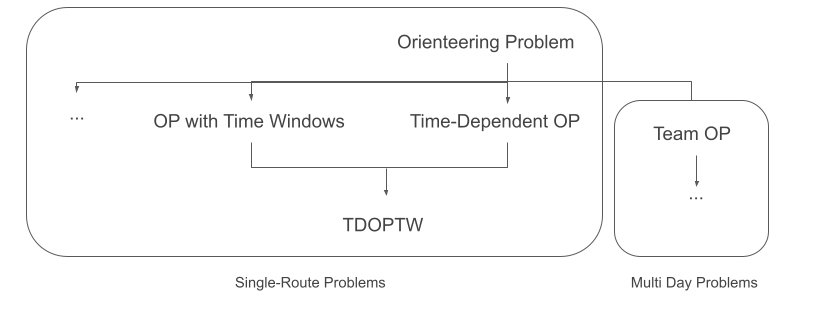
\includegraphics[width=0.5\textwidth]{TOP_graph.png}

Particle Swarm Optimisation-based (PSO) systems provide prevalent OP solutions
with fast computing time. These are bio-inspired meta-heuristic approaches in
which, in the TTDP, a particle represents a travel path. The particles aim to
optimise themselves by communicating with each other and using their velocity
property to move to the most optimal solution~\cite{RezaeeJordehi2013}. In 2010, Sevkli
et al.~\cite{Sevkli2010,Sevkli2010a} tested out two PSO variants:
Strengthened Particle Swarm Optimization (StPSO) and Discrete Strengthened
Particle Swarm Optimization (DStPSO). These two algorithms introduce pioneering
particles, which first perform a local search-based technique called Reduce
Variable Neighborhood Search (RVNS) between all the particles and then assign a
random velocity. These PSO algorithms obtains either the best or competitive
solutions compared with other algorithms such as ant colony and genetic
algorithms when tested on the Tsiligirides~\cite{Tsiligirides1984, Chen2011a} dataset.


There are numerous Evolutionary Algorithms (EA) proposed to solve OP.\@
~\cite{Kobeaga2018,Wang2008}. EAs are algorithms based on natural evolution which
use a fitness score to get to the best solution of a problem, in this case, the
TTDP~\cite{Gunawan2016}. A novel approach in 2018  by Kobeaga et al.~\cite{Kobeaga2018} was able
to find ambitious solutions for over 400 POI nodes using the steady-state
genetic algorithm. The algorithm also implements a local
search, which aims to reduce travel time. 

In 2019, Santini et al.~\cite{Santini2019} introduced a heuristic algorithm based on
adaptive extensive neighbourhood search. They evaluated their system by
comparing it with Kobeage et al.'s EA.\@ The results showed that both algorithms
find suitable solutions in a reasonable amount of time. However, the EA finds
slightly more suitable solutions, while the extensive neighbourhood search has
a lower average gap.

In real-life scenarios, POIs have time constraints that allow them to be
visited only during specific hours, such as opening and closing hours or public
holiday constraints. Traditional OP is not able to cater for such problems. A
single route variant of the OP which solves these issues is the Orienteering
Problem with Time Windows (OPTW)~\cite{Gavalas2014a}. 

Kantor et al.~\cite{Kantor1992} provided the first attempt towards the
OPTW~\cite{Vansteenwegen2011}. They developed two heuristics;
Insertion and depth-first search. The former algorithm solves the path by
selecting a POI with the highest score over-insertion cost incrementally. On
the other hand, the depth-first search algorithm gathers parallel tree-based
solutions simultaneously and iteratively adds new POIs as long as they follow a
set of constraints. Their evaluation showed significant improvements of the
second algorithm over the insertion. Most of the novel solutions of OPTW are
for the multiple route problems discussed in the upcoming sections. 

When travelling between two POIs, the travel time may depend on certain
variable time constraints such as the traffic levels and waiting time~\cite{Herzog2020}.
The Time-Dependent Orienteering Problem (TDOP) introduced by Fomin et al.
~\cite{Fomin2002} is the single route variant of OP, which considers
these scenarios since traditional OP does not~\cite{Gunawan2016}. In 2011, Abbaspour et
al.~\cite{Abbaspour2011}provide a solution for the
Time-Dependent Orienteering Problem with Time Windows, which combines the two
previously mentioned OP variants (TDOPTW).  They propose two adaptive genetic
algorithms and multi-modal shortest pathfinding evaluated in the city of
Tehran.

In 1998, Glover et al.~\cite{Glover1998} introduced a meta-heuristic approach called the
Tabu Search, and several RSs used this algorithm
~\cite{Tang2005,Sylejmani2012,Chou2021}. This optimisation technique is
advantageous when trying to escape
from a local optimum~\cite{Chou2021}. A novel approach by Chou et al.~\cite{Chou2021} aims at
tackling the Probabilistic Orienteering Problem (POP)~\cite{POP}, which
is another variant in which every path contains a cost, and the system can
access every node within a specific probability. Moreover, each node will be
available for a visit only with a certain probability. When evaluated, a simple
tabu search could compete with complex meta-heuristics showing its potential in
this field.



\subsubsection{Multiple Route Problems.}

The RSs available from what we discussed in the previous sections can only
generate a single efficient path for a tourist's holiday. The Team Orienteering
Problem (TOP)~\cite{Chao1996} is a variant of the OP, which allows for
solving the TTDP with multiple days~\cite{Sylejmani2017}. The system generates a full
itinerary for the tourist, with a maximum total score of all routes~\cite{Herzog2020}.

Several Recommender Systems use PSO-based solutions to solve the TOP
~\cite{Muthuswamy2011,Wisittipanich2020,Yu2019}
Muthuswamy et al.~\cite{Muthuswamy2011} developed a discrete version of the PSO (DPSO)
which can generate n routes
where n can be between two to four. The algorithm consists of two procedures;
Random initialisation of n-1 routes with a calculated initialisation of the nth
route based on partial randomness and the current score divided by the current
distance of the particle.  Updating the current velocity of each particle.  The
particles use RVNS and 2-opt techniques to communicate with each other as local
search techniques. The authors evaluated their work by comparing the algorithm
to seven TOP heuristics in which DPSO performed competitively across all
applied benchmark data sets~\cite{Gavalas2014a}.

A few years later, Dang et al.\ wrote another PSO inspired algorithm (PSOiA) for
the TOP.\@ They evaluated their work using an interval graph model, which showed
how to examine a more extensive search space faster~\cite{Gunawan2016}.

Besides swarm-based algorithms, A RS by Sylejmani et al.~\cite{Sylejmani2012}
used the trajectory-based tabu search to solve a Multi Constrained Team OPTW.\
Their system followed three steps in order to generate an activity plan: a new
activity is added as a node to the trip using \emph{Insert}, a node is
exchanged with a new activity using \emph{Replace} and two nodes swap with each
other using \emph{Swap}. 

Several RSs also use PSO-based solutions in novel approaches. For example, in
2019, Yu et al.~\cite{Yu2019} developed a system for the Team OPTW variant based on
selective DPSO.\@ In 2020, Wisittipanich\cite{Wisittipanich2020} presented an application of a
metaheuristic called Global Local and Near-Neighbour Particle Swarm
Optimization (GLNPSO). Wisittipanich evaluated their results using LINGO, an
optimisation program and showed excellent results.

Recently, Gama~\cite{Gama2020}  et al.\ compared their reinforcement learning with
top-performing heuristics of the TOP, such as Vansteenwegen's Iterated Local
Searchl~\cite{Vansteenwegen2009}. The authors use a Pointer network as this has been
previously to solve TSP-related problems. This study opened a different way of
tackling the TTDP and achieved production-level performance and inference
times. An advantage of this approach is that the results are probabilistic. So
it is possible to retrieve the top-n solutions and use them in a more
generalised route recommendation system.

